\documentclass[twoside,10pt,a4paper]{article}
\usepackage[utf8]{inputenc}
\usepackage[english]{babel}
\usepackage{amsmath}
\usepackage{amsfonts}
\usepackage{amssymb}
\usepackage{graphicx}

\usepackage[left=2cm,right=2cm,top=2cm,bottom=3cm]{geometry}
\usepackage{fancyvrb}
\usepackage{listings}
\usepackage{xparse}
\usepackage{tikz} % ajout de dessins LaTeX
\usepackage{graphicx}
\usepackage{float}  % alignement des figures
\usepackage{fancyhdr}
\usepackage{enumitem}
\usepackage{verbatim}
\usepackage{xcolor}

\usepackage{caption}
\usepackage{subcaption}

\pagestyle{fancy} %fancyhdr
	\fancyhf{} %fancyhdr
	\renewcommand{\sectionmark}[1]{\markboth{#1}{}}
	\fancyhead[R]{NLDCI Set 5 Questions} %INSERT TITLE HERE FOR fancyhdr
	\fancyhead[L]{\nouppercase{\leftmark}} %fancyhdr
	\cfoot{\thepage} %fancyhdr
	\setlength{\headheight}{35pt}
	\setlength{\parindent}{0pt}
	
	\definecolor{MyBlue}{HTML}{4A90E2}
	\definecolor{MyRed}{HTML}{D0021B}
	\definecolor{MyGreen}{HTML}{7ED321} % Same color use in Mathcha

\begin{titlepage}
\title{\huge \textbf{Nonlinear Dynamics \& Chaos I \\ \Large Exercice Set 5 Questions}}	%TITLE
\author{ }		%AUTHOR
\date{ }	%DATE

\end{titlepage}


\begin{document}

\maketitle

\section*{Question 1}
Consider the quadratic \textit{Duffing equation}
\begin{align*}
	\dot{u} &= v, \\
	\dot{v} &= \beta u - u^2 - \delta v,
\end{align*}
where $\delta > 0$, and $0 \leq |\beta| \ll 1$.

\begin{enumerate}[label=(\alph*)]
	\item Construct a $\beta$-dependent center manifold up to quadratic order near the origin for small $\beta$ values.
	\item Construct a stability diagram for the reduced system on the center manifold using $\beta$ as a bifurcation parameter.
\end{enumerate}


\section*{Question 2}
Consider a dynamical system that has a pair of purely imaginary eigenvalues at its fixed point for the parameter value $\mu=0$. As we have seen, a linear change of coordinates and a center manifold reduction gives the two-dimensional reduced dynamical system


\begin{align}
\label{1}
\dot{x} &= \delta(\mu)x - \omega(\mu)y + f(x, y, \mu), \\
\dot{y} &= \delta(\mu)y+\omega(\mu)x + g(x,y,\mu),
\end{align}
where $\delta(\mu)=\text{Re }\lambda(\mu)$, $\omega(\mu) = \text{Im }\lambda(\mu)$. (Here $\lambda(\mu)$ and $\bar{\lambda(\mu)}$ is the pair of complex eigenvalues that crosses the imaginary axis at $\mu=0$.)

Recall that in polar coordinates, the truncated normal form of \eqref{1} can be written as

\begin{align*}
\dot{r} &= r(d_0\mu + a_0 r^2), \\
\dot{\theta} &= \omega_0 + b_0\mu + c_0r^2,
\end{align*}

where

\begin{align*}
d_0 &= \delta'(0), \quad \omega_0 = \omega(0) \\
a_0 &= \frac{1}{16}\left[f_{xxx}+f_{xyy}+g_{xxy}+g_{yyy} \right]_{x=y=0,\mu=0} \\
	&+ \frac{1}{16\omega_0}\left[f_{xy}(f_{xx}+f_{yy}) - g_{xy}(g_{xx} + g_{yy}) - f_{xx}g_{xx}+f_{yy}g_{yy} \right]_{x=y=0, \mu=0}.
\end{align*}

These classic formulae are used in all applications where Hopf bifurcations are analyzed.

As an application of these results, consider now the stick-slip oscillator

\begin{equation*}
m\ddot{x}+c\dot{x}+kx=F_f, \qquad F_f=mg\mu_0\left(1+e^{-\beta |v_0-\dot{x}|} \right)\text{sign }(v_0-\dot{x}),
\end{equation*}

where $m$ is the mass of the oscillator, $g$ is the constant of gravity, $\beta>0$ is a constant, $\mu_0$ is the Coulomb (static) friction coefficient, $v_0$ is the speed of the belt, $x$ is the position of the mass on the belt, $c$ is the coefficient of viscous damping, and $k$ is the spring coefficient (see Fig. \ref{fig1}).

\begin{figure}[h!]
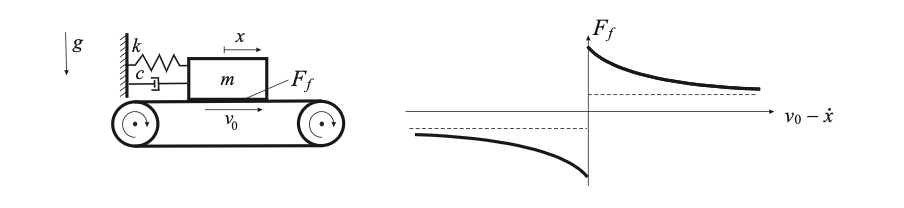
\includegraphics[width = \textwidth]{Graphics/hopf.png}\label{fig1}
\caption{Stick-slip oscillator and its dry-friction force as a function of the relative velocity between the mass and the belt.}
\label{fig1}
\end{figure}
\begin{enumerate}[label=(\alph*)]
\item Find a condition under which the system has an asymptotically stable fixed point.
\item Show that a subcritical Hopf bifurcation takes place when the above condition is violated. (Use $v_0$ as a bifurcation parameter.)
\item Calculate the approximate amplitude of the bifurcating limit cycle.
%\item Pick parameter values for which a stable limit cycle coexists with the stable equilibrium (close to the bifurcation point, i.e., for $v_0>0$ small). For these parameter values, plot trajectories in the phase space to illustrate the two competing stable behaviors. Also plot the limit cycle amplitude you obtained from your normal form calculation, and compare your numerical and analytical results. 
\end{enumerate}

\end{document}